%!TEX root = ../thesis.tex
% ******************************* Thesis Appendix A ****************************
\chapter{Knowledge Graph Statistics} 

\ifpdf
     \graphicspath{{Figs/Chapter4/}}
\else
    \graphicspath{{Chapter4/Figs/Vector/}{Chapter4/Figs/}}
\fi

\begin{figure}[H]
	\parbox{.5\linewidth}{
   		\centering
    		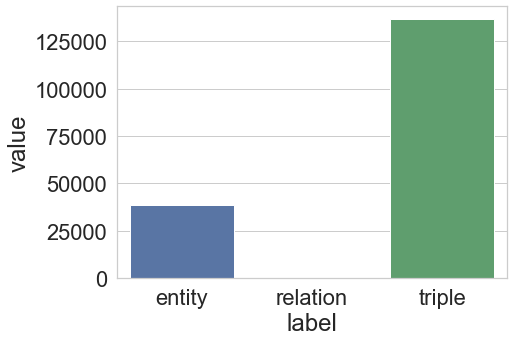
\includegraphics[width=0.45\textwidth, height=0.3\textwidth]{Wordnet_Counts}
		\captionsetup{justification=centering}
		\caption{WordNet KG count of entities, relations and facts.}
		}
	\hfill
	\parbox{.5\linewidth}{
   		\centering
    		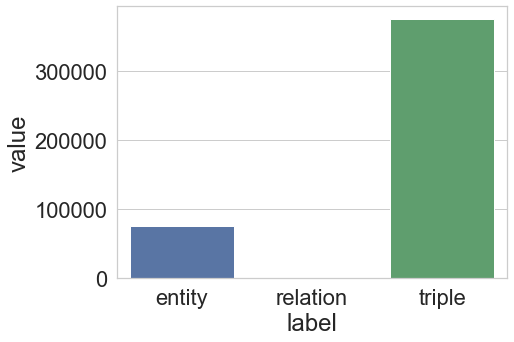
\includegraphics[width=0.45\textwidth, height=0.3\textwidth]{Freebase_Counts}
		\captionsetup{justification=centering}
		\caption{Freebase KG count of entities, relations and facts.}
		}
\end{figure}

%\section*{Windows OS}
%
%\subsection*{TeXLive package - full version}
%\begin{enumerate}
%\item	Download the TeXLive ISO (2.2GB) from\\
%\href{https://www.tug.org/texlive/}{https://www.tug.org/texlive/}
%\item	Download WinCDEmu (if you don't have a virtual drive) from \\
%\href{http://wincdemu.sysprogs.org/download/}
%{http://wincdemu.sysprogs.org/download/}
%\item	To install Windows CD Emulator follow the instructions at\\
%\href{http://wincdemu.sysprogs.org/tutorials/install/}
%{http://wincdemu.sysprogs.org/tutorials/install/}
%\item	Right click the iso and mount it using the WinCDEmu as shown in \\
%\href{http://wincdemu.sysprogs.org/tutorials/mount/}{
%http://wincdemu.sysprogs.org/tutorials/mount/}
%\item	Open your virtual drive and run setup.pl
%\end{enumerate}
%
%or
%
%\subsection*{Basic MikTeX - \TeX~ distribution}
%\begin{enumerate}
%\item	Download Basic-MiK\TeX (32bit or 64bit) from\\
%\href{http://miktex.org/download}{http://miktex.org/download}
%\item	Run the installer 
%\item	To add a new package go to Start >> All Programs >> MikTex >> Maintenance (Admin) and choose Package Manager
%\item	Select or search for packages to install
%\end{enumerate}
%
%\subsection*{TexStudio - \TeX~ editor}
%\begin{enumerate}
%\item	Download TexStudio from\\
%\href{http://texstudio.sourceforge.net/\#downloads}
%{http://texstudio.sourceforge.net/\#downloads} 
%\item	Run the installer
%\end{enumerate}
%
%\section*{Mac OS X}
%\subsection*{MacTeX - \TeX~ distribution}
%\begin{enumerate}
%\item	Download the file from\\
%\href{https://www.tug.org/mactex/}{https://www.tug.org/mactex/}
%\item	Extract and double click to run the installer. It does the entire configuration, sit back and relax.
%\end{enumerate}
%
%\subsection*{TexStudio - \TeX~ editor}
%\begin{enumerate}
%\item	Download TexStudio from\\
%\href{http://texstudio.sourceforge.net/\#downloads}
%{http://texstudio.sourceforge.net/\#downloads} 
%\item	Extract and Start
%\end{enumerate}
%
%
%\section*{Unix/Linux}
%\subsection*{TeXLive - \TeX~ distribution}
%\subsubsection*{Getting the distribution:}
%\begin{enumerate}
%\item	TexLive can be downloaded from\\
%\href{http://www.tug.org/texlive/acquire-netinstall.html}
%{http://www.tug.org/texlive/acquire-netinstall.html}.
%\item	TexLive is provided by most operating system you can use (rpm,apt-get or yum) to get TexLive distributions
%\end{enumerate}
%
%\subsubsection*{Installation}
%\begin{enumerate}
%\item	Mount the ISO file in the mnt directory
%\begin{verbatim}
%mount -t iso9660 -o ro,loop,noauto /your/texlive####.iso /mnt
%\end{verbatim}
%
%\item	Install wget on your OS (use rpm, apt-get or yum install)
%\item	Run the installer script install-tl.
%\begin{verbatim}
%	cd /your/download/directory
%	./install-tl
%\end{verbatim}
%\item	Enter command `i' for installation
%
%\item	Post-Installation configuration:\\
%\href{http://www.tug.org/texlive/doc/texlive-en/texlive-en.html\#x1-320003.4.1}
%{http://www.tug.org/texlive/doc/texlive-en/texlive-en.html\#x1-320003.4.1} 
%\item	Set the path for the directory of TexLive binaries in your .bashrc file
%\end{enumerate}
%
%\subsubsection*{For 32bit OS}
%For Bourne-compatible shells such as bash, and using Intel x86 GNU/Linux and a default directory setup as an example, the file to edit might be \begin{verbatim}
%edit $~/.bashrc file and add following lines
%PATH=/usr/local/texlive/2011/bin/i386-linux:$PATH; 
%export PATH 
%MANPATH=/usr/local/texlive/2011/texmf/doc/man:$MANPATH;
%export MANPATH 
%INFOPATH=/usr/local/texlive/2011/texmf/doc/info:$INFOPATH;
%export INFOPATH
%\end{verbatim}
%\subsubsection*{For 64bit OS}
%\begin{verbatim}
%edit $~/.bashrc file and add following lines
%PATH=/usr/local/texlive/2011/bin/x86_64-linux:$PATH;
%export PATH 
%MANPATH=/usr/local/texlive/2011/texmf/doc/man:$MANPATH;
%export MANPATH 
%INFOPATH=/usr/local/texlive/2011/texmf/doc/info:$INFOPATH;
%export INFOPATH
%
%\end{verbatim}
%
%
%
%%\subsection{Installing directly using Linux packages} 
%\subsubsection*{Fedora/RedHat/CentOS:}
%\begin{verbatim} 
%sudo yum install texlive 
%sudo yum install psutils 
%\end{verbatim}
%
%
%\subsubsection*{SUSE:}
%\begin{verbatim}
%sudo zypper install texlive
%\end{verbatim}
%
%
%\subsubsection*{Debian/Ubuntu:}
%\begin{verbatim} 
%sudo apt-get install texlive texlive-latex-extra 
%sudo apt-get install psutils
%\end{verbatim}
